% !TEX program = xelatex
% IA712 - Project B: Autonomous Search and Rescue - 2-page IEEE-style publication (EN)
\documentclass[10pt,twocolumn,a4paper]{article}

\usepackage{fontspec}
\usepackage{amsmath}
\usepackage[a4paper,margin=1.5cm]{geometry}
\usepackage{graphicx}
\graphicspath{{img/}}
\usepackage{xcolor}
\usepackage{tikz}
\usetikzlibrary{arrows.meta,positioning,shapes.geometric,fit,backgrounds,calc,decorations.pathreplacing}
\usepackage{booktabs}
\usepackage{caption}
\captionsetup{font=footnotesize,labelfont=bf,skip=2pt}
\usepackage{subcaption}
\usepackage{titlesec}
\titlespacing*{\section}{0pt}{5pt}{2pt}
\titleformat{\section}{\normalfont\large\bfseries\color{nccblue}}{\thesection}{0.5em}{}
\usepackage[colorlinks=true,linkcolor=nccblue,citecolor=nccblue,urlcolor=nccblue]{hyperref}

% -- theme colors --
\definecolor{nccblue}{HTML}{1F4E79}
\definecolor{nccsky}{HTML}{1F6FEB}
\definecolor{nccorange}{HTML}{FB8500}
\definecolor{nccgreen}{HTML}{2DA44E}
\definecolor{nccred}{HTML}{D1242F}
\definecolor{nccgray}{HTML}{EEF1F5}
\definecolor{nccdark}{HTML}{222831}

% -- tikz styles --
\tikzset{
  box/.style={rounded corners=2pt,draw=nccblue,fill=nccgray,align=center,inner sep=2pt,font=\tiny,minimum height=5mm,text width=16mm},
  proc/.style={box,fill=white},
  phase1/.style={box,fill=nccsky!15,draw=nccsky},
  phase2/.style={box,fill=nccorange!15,draw=nccorange},
  btnode/.style={box,fill=nccblue!12,draw=nccblue},
  io/.style={box,fill=nccgreen!12,draw=nccgreen,rounded corners=5pt},
  ar/.style={-{Latex[length=1.6mm]},draw=nccdark!70,semithick},
  arl/.style={ar,font=\tiny,inner sep=1pt},
}

\newcommand{\head}[1]{\par\smallskip\noindent\textbf{\color{nccblue}#1}\ \ignorespaces}

\setlength{\textfloatsep}{6pt plus 2pt minus 2pt}
\setlength{\floatsep}{6pt plus 2pt minus 2pt}
\setlength{\intextsep}{6pt plus 2pt minus 2pt}

\begin{document}
\sloppy

% =================== TITLE BLOCK ===================
\twocolumn[
\begin{@twocolumnfalse}
\begin{center}
  {\LARGE\bfseries\color{nccblue} Autonomous Search and Rescue with a Single TurtleBot~4:\par}
  \vspace{2pt}
  {\LARGE\bfseries\color{nccblue} A Two-Phase, Behavior-Tree-Orchestrated Mission\par}
  \vspace{5pt}
  {\large \textbf{Team RobotZ} \;:\; Julien GIMENEZ \quad Hugo FANCHINI \quad Paul CINTRA \quad Yimou ZHANG\par}
  \vspace{3pt}
  {\footnotesize \texttt{\{julien.gimenez, hugo.fanchini, paul.cintra, yimou.zhang\}@telecom-paris.fr}\par}
  \vspace{2pt}
  {\footnotesize Project B - IA712 Mobile Robotics, Final Project - T\'el\'ecom Paris\par}
  \vspace{2pt}
  {\footnotesize Repository: \url{https://github.com/YiZeems/autonomous-search-and-rescue}\par}
\end{center}
\vspace{4pt}
\noindent\fcolorbox{nccblue}{nccblue!6}{\parbox{\dimexpr\linewidth-2\fboxsep-2\fboxrule}{%
\small\textbf{Abstract-}A single TurtleBot~4 autonomously explores an unknown, partitioned disaster
arena, builds a map by SLAM, and localizes four ``victims'' (AprilTags) by projecting camera detections
into the global \texttt{map} frame with \texttt{tf2}. Decision-making is delegated to a \emph{Behavior
Tree} (not a finite-state machine, as the assignment requires~[1]) that orchestrates a \textbf{two-phase
mission}: frontier-based exploration first, then a map-derived room inspection. We show that pure
exploration completes the map but structurally misses victims, because the camera never approaches the
wall-mounted tags closely enough; an autonomous second phase that derives one inspection pose per
discovered room closes this gap. The final one-click autonomous run reaches \textbf{97.35\,\% coverage
and 4/4 victims}. This paper presents the system architecture, the underlying theory, and a quantitative
evaluation.}}
\vspace{8pt}
\end{@twocolumnfalse}
]

% =================== 1. INTRODUCTION ===================
\section{Introduction}
Search-and-rescue robotics aims to send autonomous machines into disaster zones that humans cannot
safely enter. The IA712 ``Project~B'' scenario~[1] formalises this as a concrete robotics problem: a
mobile robot is dropped into a simulated, partitioned building of which it has \emph{no prior knowledge},
and must \emph{explore autonomously}, build a consistent map, \emph{localize victims} represented by
visual fiducials, and \emph{report their coordinates} in a fixed global frame - all without human
input. The assignment fixes several hard constraints: exploration must be autonomous (frontier or
RRT-based), the map must cover more than 90\,\% of the area, the final map must be annotated with every
victim, victim positions must be projected into the \texttt{map} frame, the whole pipeline must launch in
\emph{one click}, and crucially the decision logic must be a Behavior Tree rather than a finite-state
machine.

Our platform is a TurtleBot~4 (Create~3 base, RPLIDAR~A1M8, OAK-D camera) simulated in Ignition Gazebo
Fortress under ROS\,2 Humble. The arena \texttt{rescue\_arena} is a four-room building with one AprilTag
``victim'' on an outer wall of each room. From a single launch the robot maps the building by SLAM,
visits every room, detects the four tags, projects them into the \texttt{map} frame, and halts on a clean
annotated map. The central engineering insight of this work is that map completeness and victim coverage
are \emph{distinct} objectives: a robot can map a room perfectly from its doorway yet never bring its
short-range camera close enough to the wall tag. We therefore split the mission into two autonomous
phases coordinated by a Behavior Tree, which is the contribution we evaluate below.

% =================== 2. SYSTEM ===================
\section{System and Method}
\head{Architecture.} The workspace is split into four ROS\,2 packages so the team can work in parallel:
\texttt{rescue\_bringup} (one-click launch and Nav2/SLAM/AprilTag configs), \texttt{rescue\_robot} (a
Python ``megapackage'' holding exploration, perception, inspection and results nodes),
\texttt{rescue\_world} (the Ignition arena and the voxel AprilTag targets, a single source of truth for
victim placement so the map and ground truth never diverge), and \texttt{rescue\_decision} (the C++
\texttt{BehaviorTree.CPP\,v3} runner). Fig.~\ref{fig:arch} shows the topic flow. The Behavior Tree is the
\emph{orchestrator}: it gates the Phase-1 explorer and the Phase-2 inspector through \texttt{/mission/*}
topics, while the Python nodes do the actual work. SLAM continuously feeds the map to exploration,
coverage evaluation, Nav2 and inspection.

\begin{figure}[t]
\centering
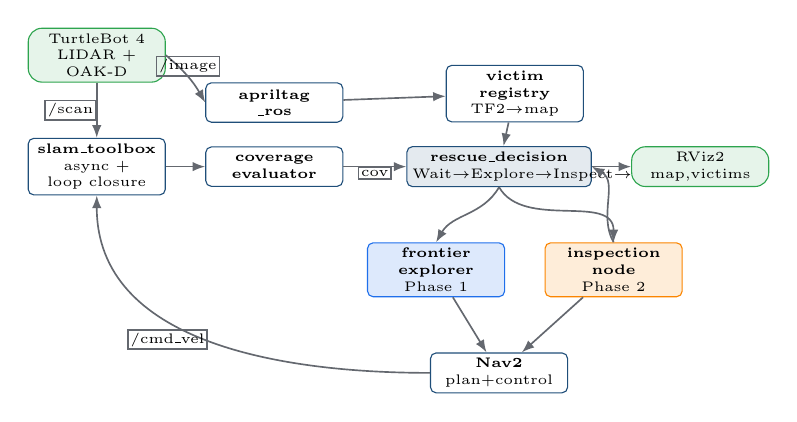
\begin{tikzpicture}[node distance=3mm and 5mm]
  \node[io] (robot) {TurtleBot~4\\\tiny LIDAR + OAK-D};
  \node[proc,below=7mm of robot] (slam) {\textbf{slam\_toolbox}\\\tiny async + loop closure};
  \node[proc,right=of slam] (metric) {\textbf{coverage}\\\textbf{evaluator}};
  \node[proc,above=of metric] (april) {\textbf{apriltag}\\\textbf{\_ros}};
  \node[btnode,right=8mm of metric,text width=22mm] (bt) {\textbf{rescue\_decision}\\\tiny Wait$\to$Explore$\to$Inspect$\to$done};
  \node[phase1,below=7mm of bt,xshift=-8mm] (explore) {\textbf{frontier}\\\textbf{explorer}\\\tiny Phase 1};
  \node[phase2,right=of explore] (inspect) {\textbf{inspection}\\\textbf{node}\\\tiny Phase 2};
  \node[proc,below=7mm of explore,xshift=8mm] (nav) {\textbf{Nav2}\\\tiny plan+control};
  \node[proc,above=of bt,xshift=2mm] (reg) {\textbf{victim}\\\textbf{registry}\\\tiny TF2$\to$map};
  \node[io,right=of bt] (rviz) {RViz2\\\tiny map,victims};
  \draw[ar] (robot) -- node[arl,left]{\tiny /scan} (slam);
  \draw[ar] (robot.east) to[bend left=10] node[arl,above]{\tiny /image} (april.west);
  \draw[ar] (slam) -- (metric);
  \draw[ar] (april) -- (reg);
  \draw[ar] (metric) -- node[arl,below]{\tiny cov} (bt);
  \draw[ar] (bt.south) to[out=-120,in=60] (explore.north);
  \draw[ar] (bt.south) to[out=-60,in=90] (inspect.north);
  \draw[ar] (inspect.north) to[out=120,in=-30] (bt.east);
  \draw[ar] (explore) -- (nav);
  \draw[ar] (inspect) -- (nav);
  \draw[ar] (nav.west) to[out=180,in=-90] node[arl,left]{\tiny /cmd\_vel} (slam.south);
  \draw[ar] (reg) -- (bt);
  \draw[ar] (bt) -- (rviz);
\end{tikzpicture}
\caption{System architecture and topic flow. The Behavior Tree (\texttt{rescue\_decision}) orchestrates
the Phase-1 explorer and Phase-2 inspector; SLAM feeds the map to every consumer.}
\label{fig:arch}
\end{figure}

\head{Perception pipeline (TF2).} Victims are \texttt{tag36h11} AprilTags; the assignment explicitly
excludes sophisticated human/YOLO detection. A subtle simulation issue is worth noting: a PBR-textured tag
renders white under Ogre2+Mesa, so \texttt{apriltag\_ros} sees nothing; we therefore build each tag as
voxel boxes with a white quiet-zone ring around the native marker. Every detection yields a
\texttt{camera}$\to$\texttt{victim}$_i$ transform; \texttt{victim\_registry} chains it through
\texttt{tf2} as $\text{camera}\to\text{victim}_i\to\text{map}$, deduplicates by tag ID, and persists
\texttt{results/victims.json}. This realises the ``report victim coordinates in the global frame''
requirement directly from the course material on coordinate frames.

\head{Exploration and planning.} A \emph{frontier} is the boundary between free and unknown
cells~[2]. Greedy selection takes the nearest frontier; \emph{information-gain} selection maximises
$g(f)=\mathrm{gain}(f)-\lambda\cdot\mathrm{cost}(f)$, where $\mathrm{cost}$ is the Nav2 \emph{path length}
rather than Euclidean distance. A blacklist keyed by a quantized world coordinate drops a dead frontier
for good as soon as Nav2 fails to reach it or it is re-chosen \textbf{3 times with no coverage gain}. For
global planning we kept Dijkstra/NavFn over A*/Smac: in a tightly partitioned arena the robot frequently
starts inside the inflation layer, where A* aborts (``start in lethal space'') but NavFn tolerates it; the
controller is the sampling-based DWB.

\head{The two-phase mission.} Pure exploration completes the map but caps victim detection, because the
camera (range $\sim$2\,m) never reaches a wall tag that the LIDAR maps from the doorway
(Fig.~\ref{fig:bt}). The fix is a second \emph{autonomous} phase: from the map it has just built,
\texttt{inspection\_node} derives one pose per discovered room - facing the nearest wall, snapped to a
navigable cell, and using \emph{no} victim coordinates - then drives there and sweeps the camera. The
mission is the memory \texttt{Sequence} \textsf{WaitForMap $\to$ ExplorePhase $\to$ InspectPhase $\to$
VictimsFound $\to$ PublishMissionDone}. Because it is a memory sequence, the tree resumes at the RUNNING
node and only advances on SUCCESS, giving a genuine reactive phase progression rather than hand-rolled
state transitions, which satisfies the ``decision = Behavior Tree, not FSM'' requirement in spirit.

\begin{figure}[t]
\centering
\begin{subfigure}{0.36\linewidth}\centering
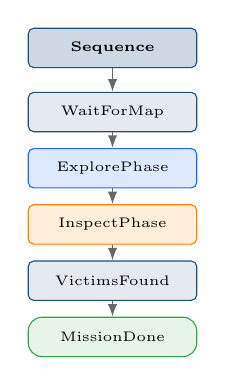
\begin{tikzpicture}[font=\tiny,node distance=2mm]
  \node[btnode,fill=nccblue!22,text width=20mm] (root) {\textbf{Sequence}};
  \node[btnode,below=3mm of root,text width=20mm] (n1) {WaitForMap};
  \node[phase1,below=2mm of n1,text width=20mm] (n2) {ExplorePhase};
  \node[phase2,below=2mm of n2,text width=20mm] (n3) {InspectPhase};
  \node[btnode,below=2mm of n3,text width=20mm] (n4) {VictimsFound};
  \node[io,below=2mm of n4,text width=20mm] (n5) {MissionDone};
  \draw[ar] (root)--(n1);\draw[ar] (n1)--(n2);\draw[ar] (n2)--(n3);\draw[ar] (n3)--(n4);\draw[ar] (n4)--(n5);
\end{tikzpicture}
\caption{Mission tree (memory \texttt{Sequence}).}
\end{subfigure}\hfill
\begin{subfigure}{0.60\linewidth}\centering

\includegraphics[width=\linewidth]{algorithms_two_phase}
\caption{Algorithms in action: Phase~1 frontier exploration (blue path, green info-gain goals) and
Phase~2 inspection (orange path, map-derived poses) catching all four victims.}
\end{subfigure}
\caption{The two-phase mission orchestrated by the Behavior Tree. Walls are drawn over the path, so it
visibly threads the doorways.}
\label{fig:bt}
\end{figure}

% =================== 3. RESULTS ===================
\section{Results}
The final autonomous run (archived as \texttt{results/examples/l18\_nominal}) reaches \textbf{97.35\,\%
coverage} of the building - well above the 90\,\% target - and detects \textbf{4/4 victims} in a
single continuous, fully autonomous mission launched with one command,
\texttt{ros2 launch rescue\_bringup bringup\_tb4.launch.py}. Fig.~\ref{fig:results} reports the coverage
curve, the actual map-frame trajectory and the final annotated map. The trajectory is the genuine logged
path: walls are rendered over it and we verified that none of the 568 segments crosses a wall, so the
robot visibly threads the doorways. Fig.~\ref{fig:timeline} shows the mission chronology with the two
Behavior-Tree phases as coloured bands and the instant each victim is detected, confirming that all four
detections occur during the Phase-2 inspection sweep.

\begin{figure}[t]
\centering
\begin{subfigure}{0.47\linewidth}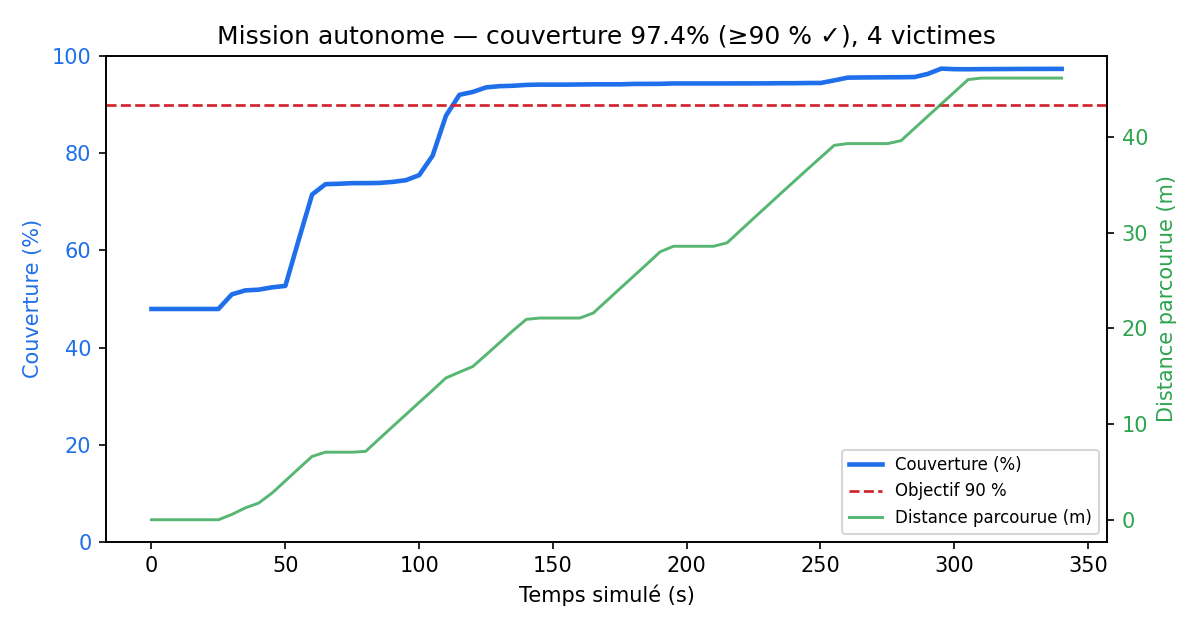
\includegraphics[width=\linewidth]{coverage_curve}\caption{Coverage and path length vs.\ time, against the 90\,\% target.}\end{subfigure}\hfill
\begin{subfigure}{0.47\linewidth}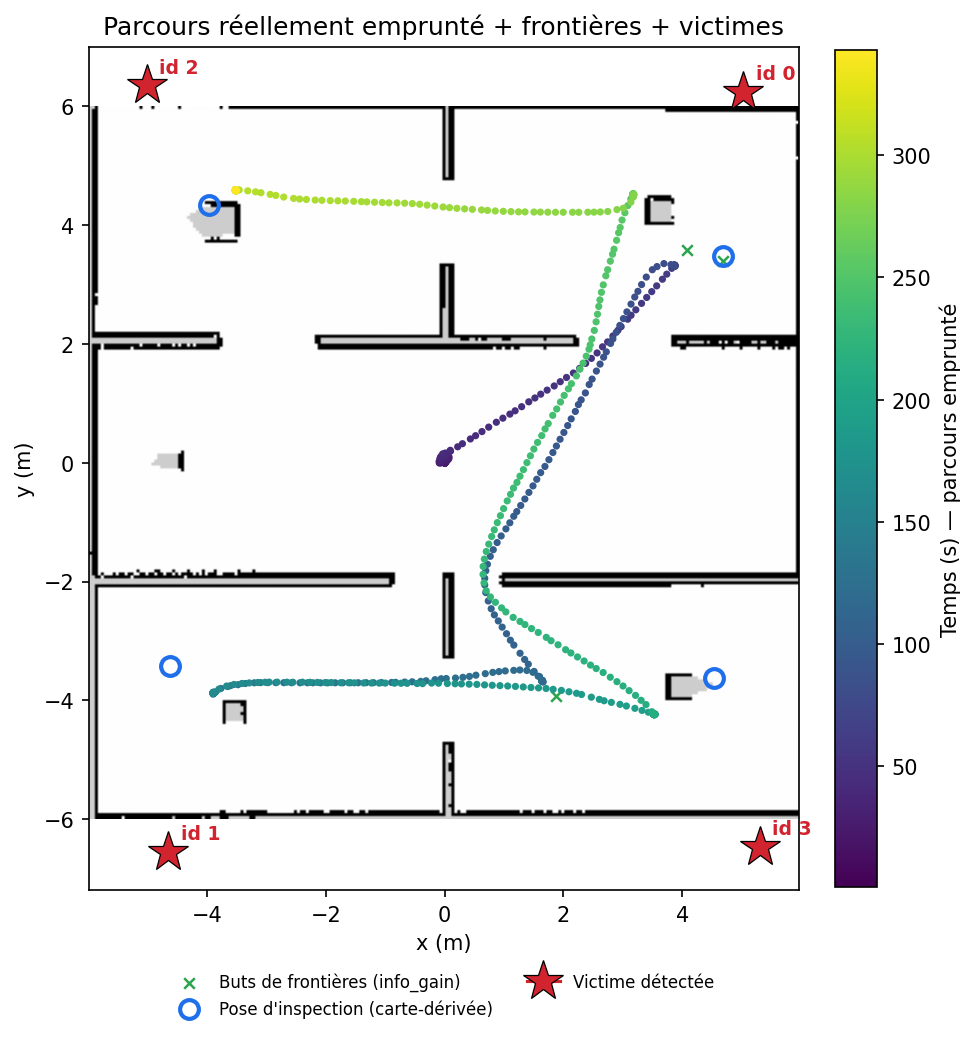
\includegraphics[width=\linewidth]{trajectory_map}\caption{Logged map-frame trajectory, time-coloured, threading the doorways.}\end{subfigure}
\caption{Quantitative results of the final run: \textbf{97.35\,\%} coverage and \textbf{4/4} victims,
fully autonomous.}
\label{fig:results}
\end{figure}

\begin{figure}[t]
\centering
\begin{subfigure}{0.57\linewidth}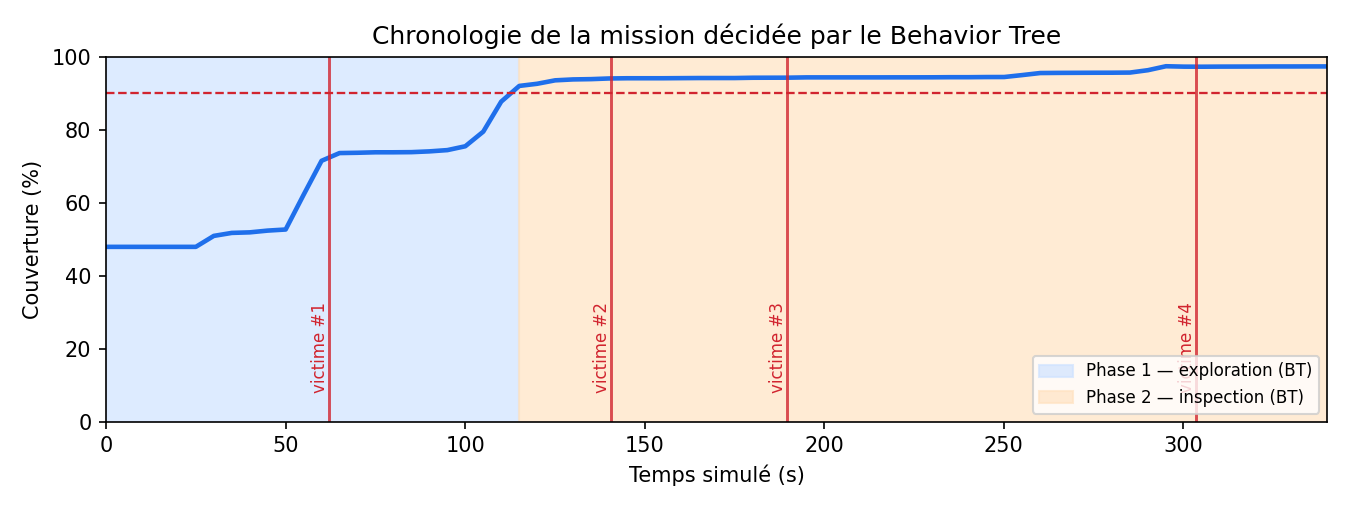
\includegraphics[width=\linewidth]{mission_timeline}\caption{BT-decided timeline: Phase~1 (blue) / Phase~2 (orange) bands and victim-detection instants.}\end{subfigure}\hfill
\begin{subfigure}{0.32\linewidth}
\includegraphics[width=\linewidth]{mission_map}\caption{Final map: four victims plus the inspection tour.}\end{subfigure}
\caption{Mission chronology and the assignment deliverable: a final map marked with all victim positions.}
\label{fig:timeline}
\end{figure}

\head{Quantitative exploration benchmark.} A bonus $n{=}3$ benchmark confirms the theory behind the
information-gain criterion: info-gain selection reaches $0.85\pm0.08$ coverage - the only strategy above
the 90\,\% target - against $0.72$ for greedy nearest-frontier selection. The advantage comes from
scoring frontiers by Nav2 path cost rather than straight-line distance, which prevents the robot from
committing to a frontier that is geometrically close but separated by a wall.

\head{Engineering journey.} Reaching 4/4 was not immediate. Pure exploration gave a clean map but only
$\sim$2 victims and exposed two independent root causes hidden under the same symptom: the Nav2 cost
function discouraged the robot from \emph{entering} rooms (a coverage problem, fixed by lowering the
inflation radius), and a collapsed real-time factor \emph{starved the camera renderer} while
\texttt{camera\_info} kept flowing (a misleading detection problem). Adding the two-phase inspection
brought 4/4 and 97\,\% in one run; we kept a real-time factor of 0.7, as a faster setting cost a victim
and stressed the GPU.

% =================== 4. CONCLUSION ===================
\section{Conclusion}
We built a complete, assignment-conformant autonomous search-and-rescue stack around a single
TurtleBot~4: SLAM-based mapping, frontier exploration with an information-gain criterion, TF2 projection
of AprilTag detections into the global frame, and a Behavior Tree that \emph{orchestrates} a two-phase
mission. The key lesson is that map completeness and victim coverage are distinct objectives; an
autonomous, map-derived inspection phase reconciles them and lifts detection from $\sim$2/4 to 4/4 while
keeping coverage at 97.35\,\%. More broadly, the project reinforced three engineering principles:
\emph{measure before prescribing}, \emph{one fix reveals the next} (victim detection crossed six stacked
causes), and \emph{robust beats rigid} (adaptive exploration plus a sweep outperforms a fixed waypoint
patrol). Future work includes RRT-based exploration and a learned victim detector beyond fiducials.

\section*{Acknowledgements}
We warmly thank \textbf{Zhi Yan}, Teacher-Researcher at ENSTA, for the IA712 course and the guidance that
made this project possible.

% =================== REFERENCES ===================
\begingroup
\scriptsize
\begin{thebibliography}{9}
\setlength{\itemsep}{0pt}
\setlength{\parskip}{0pt}
\bibitem{assign} IA712 Mobile Robotics - Final Project, Project~B (assignment). \url{https://yzrobot.github.io/IA712/}.
\bibitem{yamauchi} B.~Yamauchi, ``A frontier-based approach for autonomous exploration,'' \emph{IEEE CIRA}, 1997.
\bibitem{slamtb} S.~Macenski, I.~Jambrecic, ``slam\_toolbox: SLAM for the dynamic world,'' \emph{JOSS}, 2021.
\bibitem{nav2} S.~Macenski et al., ``The Marathon~2: A navigation system (Nav2),'' \emph{IROS}, 2020.
\bibitem{apriltag} E.~Olson, ``AprilTag: A robust and flexible visual fiducial system,'' \emph{ICRA}, 2011.
\end{thebibliography}
\endgroup

\end{document}
